\section{Verification and Validation}
In this chapter, we want to describe applicable tests to analyze the effect of the \emph{wall-avoid-distance} parameter to the output of the TEST-model. It shall be verified, that we see no overlapping and that the crowd shows typical phenomena, like lane-formation \citep{ZhangQ2011}. Following our set of tests, we will then validate the TEST-model to produce the pedestrian flow in bottleneck experiments, corresponding to empirical data. This verification is widely considered ao the most important criterion to validate simulation results \citep{Seyfried2008}.  We will further compare the trajectories with a different model, one using automated triangulation to assist routing. The last test is a mere stress test to the model. We want to see how the model performes in an evacuation setting with a large, crowded geometry.

\subsection{Basic Tests}
%The validation of a model is a complex task and makes up a separate research field. Researchers in the field of Civil Engineering are working on various approaches on how to validate a model. The research group, CST -  Pedestrian Dynamics and Traffic Simulation, is developing a set of test-cases any serious model should aim to pass. Tests include the behavior of a single moving agent passing static objects like a dummy agent or an obstacle. (see figure \ref{test01})

%The TEST-model, implemented in its current state in the simulation-suit JuPedSim\citep{jupedsim}, passed applicable tests and it was shown, that the basic mechanics of the routing are working as specified. Yet to complete validation of the model, the floorfield needs to support multiple destinations.



\begin{figure}[h!]
\includegraphics[width=1.\textwidth]{pics/Testcases01}
\caption{Testcase: Orange agent should pass the (static) blue agent.}
\vspace{1cm}
\includegraphics[width=1.\textwidth]{pics/Testcases02}
\caption{Testcase: Orange agent should pass the (static) blue obstacle.}
\label{test01}
\end{figure} 

\subsection{Variation of the Parameter}
\begin{figure}[h!]
\subfigure{\includegraphics[width=1.\textwidth]{pics/Role12_02}}
\subfigure{\includegraphics[width=1.\textwidth]{pics/Role12_16}}
\caption{Bottleneck Experiment:\\above: width: $1.2\,m$, wall-avoid-distance: $0.0\,m$\\below: width: $1.2\,m$, wall-avoid-distance: $1.6\,m$}
\label{varyWAD}
\end{figure}
We take special interest in the following test-case, as it validates the model to yield a fundamental diagram like seen in real world experiments:
The tests demands to simulate a bottleneck experiment several times. This is to be repeated for various bottleneck-widths. The calculated flow through the bottleneck shall match the empirical data.
We have conducted this test for various \emph{wall-avoid-distance} parameter and want to analyze the change in the flow. It can be seen, that the more the agents will gear to avoid obstacles and walls, the lesser the flow will become (see \ref{funddiag}). This result is expectable. It was also shown, that without the enhancement of the floor-field, few agents did \emph{not} pass the bottleneck, but got caught inside of walls.
\begin{figure}[h!]
\subfigure{\includegraphics[width=1.\textwidth]{pics/Role14_04}}
\subfigure{\includegraphics[width=1.\textwidth]{pics/Role25_04}}
\caption{Bottleneck Experiment:\\above: width: $1.4\,m$, wall-avoid-distance: $0.4\,m$\\below: width: $2.5\,m$, wall-avoid-distance: $0.4\,m$}
\label{varyWidth}
\end{figure}
%\begin{figure}[h!]
%\includegraphics[width=1.\textwidth]{pics/Role12_04}
%\caption{Bottleneck Experiment: \\width: $1.2\,m$, wall-avoid-distance: $0.4\,m$}
%\label{funddiag}
%\end{figure}
%
%\begin{figure}[h!]
%\includegraphics[width=1.\textwidth]{pics/Role12_08}
%\caption{Bottleneck Experiment: \\width: $1.2\,m$, wall-avoid-distance: $0.8\,m$}
%\label{funddiag}
%\end{figure}
%
%\begin{figure}[h!]
%\includegraphics[width=1.\textwidth]{pics/Role12_16}
%\caption{Bottleneck Experiment: \\width: $1.2\,m$, wall-avoid-distance: $1.6\,m$}
%\label{funddiag}
%\end{figure}

\begin{figure}[h!]
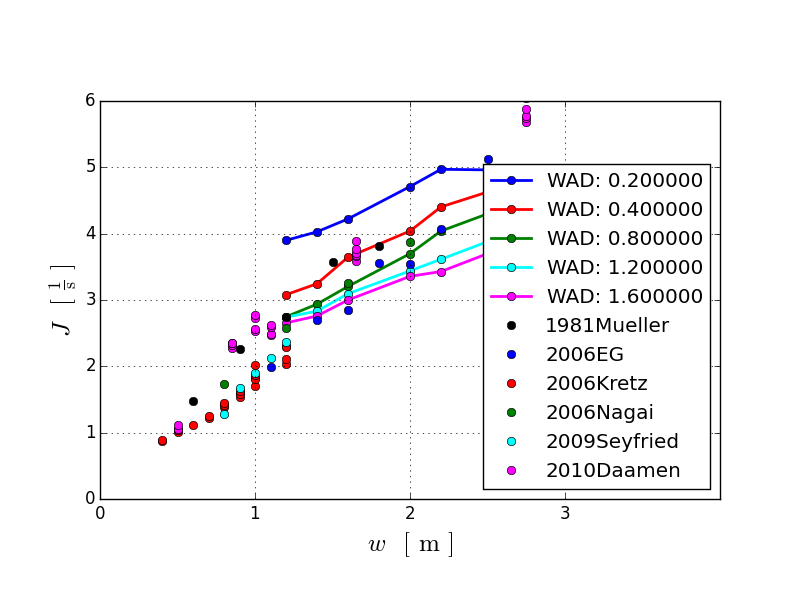
\includegraphics[width=1.\textwidth]{pics/sim_flow_vs_experimental_data}
\caption{Fundamental diagram with empiric data and simulation results}
\label{funddiag}
\end{figure}
\subsection{Laneformation}
\begin{figure}[h!]
\subfigure{\includegraphics[width=.49\textwidth]{pics/corner0}}
\subfigure{\includegraphics[width=.49\textwidth]{pics/corner1}}
\subfigure{\includegraphics[width=.49\textwidth]{pics/corner2}}
\subfigure{\includegraphics[width=.49\textwidth]{pics/corner3}}
\subfigure{\includegraphics[width=.49\textwidth]{pics/corner4}}
\subfigure{\includegraphics[width=.49\textwidth]{pics/corner5}}
\caption{Bottleneck-Corner Experiment: After the bottleneck, agents pass the corner.}
\label{funddiag}
\end{figure}